\documentclass[a4paper,12pt, oneside]{article}

\title{\textbf{Elaborato per il corso Basi di dati} \\ \large A.A 2023/2024 \\ Progetto di una base di dati per la vendita di pizze}
\author{Gabos Norbert \\ 0000970451 \\ tiberiunorbert.gabos@studio.unibo.it }
\date{}

\usepackage[T1]{fontenc}
\usepackage[utf8]{inputenc}
\usepackage[italian]{babel}
\pagestyle{plain}
\usepackage{graphicx}
\usepackage[table,xcdraw]{xcolor}
\usepackage{tabularx}
\usepackage{ragged2e}               % migliora la formattazione del testo all'interno delle celle
\renewcommand{\arraystretch}{1.5}   % aggiunge margine alle celle
\graphicspath{{images/}}

\begin{document}

\maketitle

\newpage
\tableofcontents{}
\newpage

\section{Analisi dei requisiti}

Si vuole realizzare un database per la gestione automatica della vendita
delle pizze. Pertanto la base di dati dovrà immagazzinare i dati e gli
clienti dei loro ordini, nonché dare la possibilità al venditore di
inserire o modificare le proprie pizze.

\subsection{Intervista}

Si prevede la gestione della clientela del negozio registrando il nome,
il cognome, l'email, il numero di telefono e l'indirizzo di ciascun
individuo. Ogni cliente deve poter effettuare il proprio ordine con un
limite massimo di 10 pizze. È consentito effettuare al massimo 4 ordini
ogni mezz'ora per garantire la consegna puntuale negli orari successivi.

Inoltre, il cliente potrà scegliere se farsi recapitare le pizze a casa
propria o se desidera ritirarle personalmente. Nel primo caso, è
necessario richiedere all'utente l'indirizzo di consegna.

I clienti devono essere in grado di prenotare un tavolo per quante
persone desiderano, ma non è permesso prenotare più di un tavolo ogni
mezz'ora. Inoltre, non possono esserci più di 10 tavoli prenotati
contemporaneamente per garantire la disponibilità di posti per i
clienti senza prenotazione.

Si desidera mantenere uno storico degli ordini di ciascun utente per
consentire al proprietario di stimare la domanda dei propri prodotti.
Gli utenti devono poter visualizzare l'elenco di tutti i loro ordini e
avere la possibilità di modificarli o cancellare il proprio account. In
caso di cancellazione dell'account di un cliente, devono essere
eliminati tutti i dati relativi alle operazioni effettuate, inclusi
ordini e altre attività future, per garantire la privacy degli
individui.

Ogni pizza deve appartenere a una categoria, tra cui "Pizze classiche",
"Pizze speciali" e "Impasto napoletano". Ciascuna pizza è caratterizzata
da un prezzo, un nome e una lista di ingredienti e allergeni, come
latticini, noci, uova, ecc.

Infine, è essenziale monitorare le attività dei pizzaioli, che devono
poter modificare pizze e ingredienti, eliminare quelli esistenti o
aggiungerne di nuovi. Possono anche consultare il portale per
visualizzare la classifica delle pizze più vendute e meno vendute.
Cosa più importante, è necessario che esista una pagina dove poter
visualizzare tutti gli ordini ancora non processati da utilizzare 
per sapere qual'è il prossimo ordine da preparare.
Ciò è utile per apportare eventuali modifiche al menu alla fine
dell'anno, come la modifica o la cancellazione di alcune pizze.

\begin{figure}[ht]
    \centering
    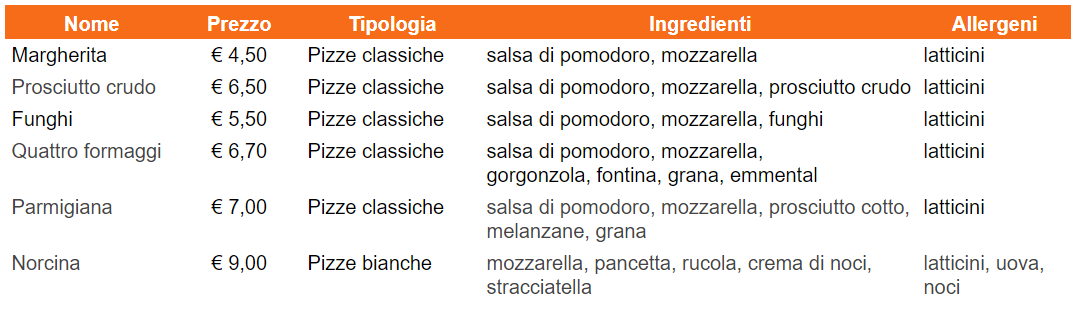
\includegraphics[width=1\textwidth]{esempio_pizze.png}
    \caption{Esempio dell'elenco di pizze.}
    \label{fig:esempio_pizze}
\end{figure}

\subsection{Estrazione dei concetti principali}

Dopo aver esaminato e compreso i requisiti, si procede con la redazione
di un testo che sintetizza tutti i concetti, concentrandosi in
particolare sull'estrazione dei principali e sulla rimozione delle
ambiguità individuate in precedenza.

TODO: Aggiungere immagine con tavella di cosa fa ogni entità principale

\begin{quote}

Per ogni cliente, è essenziale registrare il proprio nome, cognome,
numero di telefono, indirizzo email, una password per il login e un
identificativo univoco assegnato al momento della creazione
dell'account. Ciascun cliente avrà accesso a un listino completo delle
pizze e potrà selezionare quelle desiderate per aggiungerle al proprio
ordine. L'applicazione gestirà integralmente la funzione del carrello,
salvando eventuali modifiche sul dispositivo dell'utente.

Gli ordini saranno catalogati in intervalli di 30 minuti,
dall'orario di apertura a quello di chiusura, con limitazioni sia sul
numero complessivo di ordini che sul numero di pizze per ogni ordine.
Gli ordini possono essere di due tipi: consegna a domicilio o ritiro
dell'ordine; nel primo caso, è necessario memorizzare anche
l'indirizzo di recapito. Ogni utente potrà visualizzare la propria
cronologia degli ordini, ma solo il proprietario avrà accesso a tutti
gli ordini effettuati.

Ciascun tavolo deve possedere un identificatore per evitare che più
clienti prenotino lo stesso tavolo contemporaneamente; inoltre, non
possono esserci più di 10 prenotazioni a mezz'ora, e un cliente non
può prenotare più di un tavolo in una determinata fascia oraria.

Per ogni pizza, è necessario memorizzare il nome come identificatore
unico, il tipo, gli ingredienti, gli allergeni e il prezzo. Il
proprietario avrà la capacità di visualizzare e modificare tutte le
informazioni relative a ciascuna pizza. Infine, avrà la possibilità
di consultare una classifica contenente le 5 pizze più vendute e
meno vendute.

\end{quote}

Elenco delle principali azioni richieste:
\begin{enumerate}
    \item Inserimento di un nuovo cliente
    \item Inserimento di un socio
    \item Creazione di un ordine
    \item Prenotazione di un tavolo
    \item Aggiunta di una pizza
    \item Modifica delle caratteristiche di una pizza
    \item Aggiunta di un ingrediente nuovo
    \item Eliminazione di un ingrediente
    \item Visualizzazione delle pizze con relativi dettagli
    \item Visualizzazione degli ordini dei relativi clienti
    \item Visualizzazione della classifica delle pizze più vendute
\end{enumerate}

\section{Progettazione Concettuale}
\subsection{Schema scheletro}

Per l'entità \textbf{Cliente}, ho scelto di modellarla come una
generalizzazione, insieme a \textbf{Proprietario}, di \textbf{Utente}.

TODO: inserire immagine

Dall'analisi del dominio emerge che è possibile effettuare solo un
numero limitato di ordini in una determinata fascia oraria. Pertanto,
ho introdotto le entità \textbf{Fascia oraria} e \textbf{Ordine},
con un limite di 4 istanze per ogni fascia oraria. Inoltre, ho
stabilito che un cliente non può effettuare più di un ordine a mezz'ora.
Per gestire questa limitazione, l'entità \textbf{Ordine} è
identificata da una data, dalla fascia oraria e dall'ID del cliente,
evitando così che io possa effettuare ordini multipli e superare il
limite imposto. Inoltre, l'entità \textbf{Ordine} ha due sottoclassi,
\textbf{Ordine da ritirare} e \textbf{Ordine da consegnare}, con
quest'ultima che richiede un indirizzo per la consegna.

TODO: inserire immagine

Per quanto riguarda l'entità \textbf{Prenotazione tavolo}, la
situazione è più complessa. Ogni tavolo può essere prenotato solo una
volta durante una fascia oraria, e contemporaneamente, non posso
prenotare più di un tavolo per la stessa fascia oraria. Come soluzione,
ho pensato di utilizzare una chiave duplice: la prima comprende la data
della prenotazione, l'identificatore del tavolo e la fascia oraria,
mentre la seconda comprende la data della prenotazione,
l'identificatore dell'utente e la fascia oraria. In questo modo, tutti
i vincoli precedenti sono stati soddisfatti.

TODO: inserire immagine

Per quanto riguarda l'entità \textbf{Pizze}, ciascuna pizza memorizza
un prezzo e un nome che la identifica. Ho anche introdotto l'entità
\textbf{Tipo pizza}, che rappresenta il tipo di pizza identificato dal
proprio nome. Ogni pizza è composta da un numero di ingredienti, quindi
ho creato l'entità \textbf{Ingrediente}, che contiene il proprio nome
come identificatore e una descrizione. Infine, ogni ingrediente ha il
proprio allergene, modellato dall'entità \textbf{Allergene}.

TODO: inserire immagine

\subsection{Schema finale}

TODO: inserire immagine

\newpage
\section{Progettazione Logica}
\subsection{Stima del volume dei dati}

\begin{table}[ht]
\begin{tabularx}{1\textwidth}{>{\RaggedRight\arraybackslash}X>{\Centering\arraybackslash}X>{\Centering\arraybackslash}X}
    \rowcolor[HTML]{f66c19} 
    \textcolor{white}{Concetto} & \textcolor{white}{Costrutto} & \textcolor{white}{Volume} \\ \hline
    \rowcolor[HTML]{FFFFFF} 
    Cliente & E & 1000 \\ \hline
    \rowcolor[HTML]{FFFFFF} 
    Proprietario & E & 1 \\ \hline
    \rowcolor[HTML]{FFFFFF} 
    Effettuazione & R & 250000 \\ \hline
    \rowcolor[HTML]{FFFFFF} 
    Ordine da ritirare & E & 150000 \\ \hline
    \rowcolor[HTML]{FFFFFF}
    Ordine da consegnare & E & 100000 \\ \hline
    \rowcolor[HTML]{FFFFFF} 
    Associato a & R & 250000 \\ \hline
    \rowcolor[HTML]{FFFFFF} 
    Fascia oraria & E & 16 \\ \hline
    \rowcolor[HTML]{FFFFFF} 
    Pianificazione prenotazioni & R & 50000 \\ \hline
    \rowcolor[HTML]{FFFFFF} 
    Prenotazione tavolo & E & 50000 \\ \hline
    \rowcolor[HTML]{FFFFFF} 
    Riservazione & R & 50000 \\ \hline
    \rowcolor[HTML]{FFFFFF} 
    Tavolo & E & 30 \\ \hline
    \rowcolor[HTML]{FFFFFF} 
    Richiesta & R & 50000 \\ \hline
    \rowcolor[HTML]{FFFFFF} 
    Comprende & R & 250000 \\ \hline
    \rowcolor[HTML]{FFFFFF} 
    Pizza & E & 90 \\ \hline
    \rowcolor[HTML]{FFFFFF} 
    Tipologia & R & 90 \\ \hline
    \rowcolor[HTML]{FFFFFF} 
    Tipo pizza & E & 3 \\ \hline
    \rowcolor[HTML]{FFFFFF} 
    Composizione & R & 450 \\ \hline
    \rowcolor[HTML]{FFFFFF} 
    Ingrediente & E & 45
\end{tabularx}
\end{table}

\begin{table}[ht]
\begin{tabularx}{1\textwidth}{>{\RaggedRight\arraybackslash}X>{\Centering\arraybackslash}X>{\Centering\arraybackslash}X}
    \rowcolor[HTML]{f66c19} 
    \textcolor{white}{Concetto} & \textcolor{white}{Costrutto} & \textcolor{white}{Volume} \\ \hline
    \rowcolor[HTML]{FFFFFF} 
    Contiene & R & 45 \\ \hline
    \rowcolor[HTML]{FFFFFF} 
    Allergene & E & 5
\end{tabularx}
\end{table}

\subsection{Descrizione delle operazioni principali e stima della loro frequenza}

Le attività da eseguire coincidono con quelle precedentemente
dettagliate durante la fase di analisi. Di seguito è presente
una tabella che fornisce la loro descrizione e la frequenza
associata:

\begin{table}[ht]
\begin{tabularx}{\textwidth}{>{\hsize=0.2\hsize\RaggedRight\arraybackslash}X>{\hsize=1.8\hsize\RaggedRight\arraybackslash}X>{\RaggedRight\arraybackslash}X}
    \rowcolor[HTML]{f66c19} 
    \textcolor{white}{Num} & \textcolor{white}{Operazione} & \textcolor{white}{Frequenza} \\ \hline
    \rowcolor[HTML]{FFFFFF} 
    1 & Inserimento di un nuovo cliente & 1 alla settimana \\ \hline
    \rowcolor[HTML]{FFFFFF} 
    2 & Inserimento di un socio & 1 all'anno \\ \hline
    \rowcolor[HTML]{FFFFFF} 
    3 & Creazione di un ordine & 64 al giorno \\ \hline
    \rowcolor[HTML]{FFFFFF} 
    4 & Prenotazione di un tavolo & 80 al giorno \\ \hline
    \rowcolor[HTML]{FFFFFF} 
    5 & Aggiunta di una pizza & 10 all'anno \\ \hline
    \rowcolor[HTML]{FFFFFF} 
    6 & Modifica delle caratteristiche di una pizza & 20 al mese \\ \hline
    \rowcolor[HTML]{FFFFFF} 
    7 & Aggiunta di un ingrediente nuovo & 2 all'anno \\ \hline
    \rowcolor[HTML]{FFFFFF}  
    8 & Visualizzazione delle pizze con relativi dettagli & 300 al giorno \\ \hline
    \rowcolor[HTML]{FFFFFF} 
    9 & Visualizzazione degli ordini dei relativi clienti & 20 al giorno \\ \hline
    \rowcolor[HTML]{FFFFFF} 
    10 & Visualizzazione della classifica delle pizze più vendute & 2 all'anno
\end{tabularx}
\end{table}

\subsection{Schemi di navigazioni e tabelle degli accessi}

Dopo aver analizzato il volume dei dati e associato ogni
richiesta operativa alla sua frequenza e tipologia
corrispondente, si procede con la creazione delle tabelle
degli accessi e dei relativi schemi di navigazione per
ciascuna operazione. È importante notare che le operazioni di
scrittura avranno un costo doppio rispetto a quelle di
lettura.

\paragraph{OP 1 - Inserimento di un nuovo cliente}

\hphantom{A}    % se no la tabella si sposta sopra il paragrafo

\begin{table}[h]
\begin{tabularx}{\textwidth}{>{\RaggedRight\arraybackslash}X>{\RaggedRight\arraybackslash}X>{\RaggedRight\arraybackslash}X>{\RaggedRight\arraybackslash}X}
    \rowcolor[HTML]{f66c19} 
    \textcolor{white}{Concetto} & \textcolor{white}{Construtto} & \textcolor{white}{Accessi} & \textcolor{white}{Tipo} \\ \hline
    \rowcolor[HTML]{FFFFFF} 
    Cliente & E & 1 & S \\ \hline
    \rowcolor[HTML]{FFFFFF} 
    \multicolumn{4}{c}{\textbf{Totale}: 1S → 1 alla settimana = (1 x 2) x 1 / 7 = \textbf{0,285}}
\end{tabularx}
\end{table}

\paragraph{OP 2 - Inserimento di un socio}

\hphantom{A}    % se no la tabella si sposta sopra il paragrafo

\begin{table}[h]
\begin{tabularx}{\textwidth}{>{\RaggedRight\arraybackslash}X>{\RaggedRight\arraybackslash}X>{\RaggedRight\arraybackslash}X>{\RaggedRight\arraybackslash}X}
    \rowcolor[HTML]{f66c19} 
    \textcolor{white}{Concetto} & \textcolor{white}{Construtto} & \textcolor{white}{Accessi} & \textcolor{white}{Tipo} \\ \hline
    \rowcolor[HTML]{FFFFFF} 
    Proprietario & E & 1 & S \\ \hline
    \rowcolor[HTML]{FFFFFF} 
    \multicolumn{4}{c}{\textbf{Totale}: 1S → 1 all'anno = (1 x 2) x 1 / 365 = \textbf{0,005}}
\end{tabularx}
\end{table}

\paragraph{OP 3 - Creazione di un ordine}

\hphantom{A}\\    % se no la tabella si sposta sopra il paragrafo

TODO: L'id dell'utente e l'id di ogni pizza si sanno gia. Si fa una lettura su fascia oraria per vedere se c'è disponibilità
e 64 ordini al gionro, perche 4 ogni mezz'ora...

\begin{table}[h]
\begin{tabularx}{\textwidth}{>{\RaggedRight\arraybackslash}X>{\RaggedRight\arraybackslash}X>{\RaggedRight\arraybackslash}X>{\RaggedRight\arraybackslash}X}
    \rowcolor[HTML]{f66c19} 
    \textcolor{white}{Concetto} & \textcolor{white}{Construtto} & \textcolor{white}{Accessi} & \textcolor{white}{Tipo} \\ \hline
    \rowcolor[HTML]{FFFFFF} 
    Ordine & E & 1 & S \\ \hline
    \rowcolor[HTML]{FFFFFF} 
    Comprende & R & 5 & S \\ \hline
    \rowcolor[HTML]{FFFFFF} 
    Effettuazione & R & 1 & S \\ \hline
    \rowcolor[HTML]{FFFFFF} 
    Associato a & R & 1 & S \\ \hline
    \rowcolor[HTML]{FFFFFF} 
    Fascia oraria & E & 16 & L \\ \hline
    \rowcolor[HTML]{FFFFFF} 
    \multicolumn{4}{c}{\textbf{Totale}: 8S + 16L → 64 al giorno = (8 x 2) + (16 x 1) x 64 = \textbf{1040}}
\end{tabularx}
\end{table}

\paragraph{OP 4 - Prenotazione di un tavolo}

\hphantom{A}\\    % se no la tabella si sposta sopra il paragrafo

TODO: l'id dell'utente lo so gia...

\begin{table}[h]
\begin{tabularx}{\textwidth}{>{\RaggedRight\arraybackslash}X>{\RaggedRight\arraybackslash}X>{\RaggedRight\arraybackslash}X>{\RaggedRight\arraybackslash}X}
    \rowcolor[HTML]{f66c19} 
    \textcolor{white}{Concetto} & \textcolor{white}{Construtto} & \textcolor{white}{Accessi} & \textcolor{white}{Tipo} \\ \hline
    \rowcolor[HTML]{FFFFFF} 
    Prenotazione tavolo & E & 1 & S \\ \hline
    \rowcolor[HTML]{FFFFFF} 
    Richiesta & R & 1 & S \\ \hline
    \rowcolor[HTML]{FFFFFF} 
    Riservazione & R & 1 & S \\ \hline
    \rowcolor[HTML]{FFFFFF} 
    Tavolo & E & 30 & L \\ \hline
    \rowcolor[HTML]{FFFFFF} 
    Pianificazione prenotazioni & R & 1 & S \\ \hline
    \rowcolor[HTML]{FFFFFF} 
    Fascia oraria & E & 16 & L \\ \hline
    \rowcolor[HTML]{FFFFFF} 
    \multicolumn{4}{c}{\textbf{Totale}: 4S + 46L → 80 al giorno = (4 x 2) + (46 x 1) x 80 = \textbf{3688}}
\end{tabularx}
\end{table}

\paragraph{OP 5 - Aggiunta di una pizza}

A

\paragraph{OP 6 - Modifica delle caratteristiche di una pizza}

A

\paragraph{OP 7 - Aggiunta di un ingrediente nuovo}

A

\paragraph{OP 8 - Visualizzazione delle pizze con relativi dettagli}

A

\paragraph{OP 9 - Visualizzazione degli ordini dei relativi clienti}

A

\paragraph{OP 10 - Visualizzazione della classifica delle pizze più vendute}

A

\subsection{Raffinamento dello schema}
\subsection{Analisi delle ridondanze}
\subsection{Traduzione di entità e associazioni in relazioni}
\subsection{Schema relazionale finale}
\subsection{Traduzione delle operazioni in query SQL}

\section{Progettazione dell'applicazione}
\subsection{Descrizione dell'architettura dell'applicazione realizzata}

\end{document}
